\clearpage



\begin{appendix}
\hypertarget{annexes}{%
\section{Annexes}\label{annexes}}

\hypertarget{annexe-a-erratum-de-larticle-why-psychologists-should-by-default-use-welchs-t-test-instead-of-students-t-test-chapitre-2}{%
\subsection{\texorpdfstring{Annexe A: erratum de l'article ``Why
psychologists Should by Default Use Welch's \emph{t}-test Instead of
Student's \emph{t}-test'' (Chapitre
2)}{Annexe A: erratum de l'article ``Why psychologists Should by Default Use Welch's t-test Instead of Student's t-test'' (Chapitre 2)}}\label{annexe-a-erratum-de-larticle-why-psychologists-should-by-default-use-welchs-t-test-instead-of-students-t-test-chapitre-2}}

\hypertarget{mise-en-forme-et-notations}{%
\subsubsection{Mise en forme et
Notations}\label{mise-en-forme-et-notations}}

Les lettres utilisées pour décrire les statistiques (test-\(t\) ou
test-\(F\)) doivent toujours être inscrites en \emph{italique}. Or,
cela a été omis Ã~ plusieurs reprises dans l'article. Par exemple, il
aurait fallu écrire:\\
- p.9: ``\ldots{} as the Mann-Whitney \(U\)-test\ldots{}'' au lieu de
``\ldots{} as the Mann-Whitney U-test\ldots{}'';\\
- p.9: ``\(F\)-ratio test'' au lieu de ``F-ratio test''.

Certaines notations mathématiques auraient également dû être
indiquées en italique. Par exemple, Ã~ la p.9, il aurait fallu
écrire:\\
- ``\(x_{ij}\)'' au lieu de ``\(\mathrm{x_{ij}}\)'';\\
- \textbar{}\(x_{ij}-\hat{\theta_j}\)\textbar{} au lieu de
\textbar{}\(\mathrm{x_{ij}-\hat{\theta_j}}\)\textbar.

Par ailleurs, il est très important d'être consistant dans le choix
des notations mathématiques, afin d'éviter d'embrouiller le lecteur.
Or, nous n'avons pas toujours respecté cela. Par exemple, nous avons
utilisé plusieurs notations différentes pour décrire l'écart-type et
la variance. Par exemple:\\
- p.9: nous utilisons respectivement SD1 et SD2 pour décrire
l'écart-type de chaque groupe;\\
- p.11 (équation 1): nous utilisons respectivement \(S^2_1\) et
\(S^2_2\) pour décrire la variance de chaque groupe;\\
- p.12 (équation 4): nous utilisons respectivement \(s^2_1\) et
\(s^2_2\) (lettres minuscules) pour décrire la variance de chaque
groupe.

C'est d'autant plus problématique qu'il y a parfois même des
inconsistances entre les notations utilisées dans les formules et
celles utilisées dans les légendes des formules. Par exemple, nous
spécifions p.11 que dans l'équation 1, \(s^2_1\) et \(s^2_2\) (lettres
minuscules) représentent les estimations de variance de chaque groupe
indépendant, alors qu'en réalité, les estimations des variances sont
représentées par \(S^2_1\) et \(S^2_2\) (lettres majuscules) dans
l'équation 1.

\hypertarget{fautes-de-frappe}{%
\subsubsection{Faute(s) de frappe}\label{fautes-de-frappe}}

\begin{itemize}
\tightlist
\item
  p.13: ``see \sout{v} \textbf{Figure} 2a''.
\end{itemize}

\newpage

\hypertarget{annexe-b-erratum-de-larticle-taking-parametric-assumptions-very-seriously-arguments-for-the-use-of-welchuxe2s-f-test-instead-of-the-classical-f-test-in-one-way-anova-chapitre-3}{%
\subsection{\texorpdfstring{Annexe B: erratum de l'article ``Taking
parametric assumptions very seriously: Arguments for the Use of
Welch’s \emph{F}-test instead of the Classical \emph{F}-test in
One-Way ANOVA'' (Chapitre
3)}{Annexe B: erratum de l'article ``Taking parametric assumptions very seriously: Arguments for the Use of Welch’s F-test instead of the Classical F-test in One-Way ANOVA'' (Chapitre 3)}}\label{annexe-b-erratum-de-larticle-taking-parametric-assumptions-very-seriously-arguments-for-the-use-of-welchuxe2s-f-test-instead-of-the-classical-f-test-in-one-way-anova-chapitre-3}}

\hypertarget{mise-en-forme-et-notations-1}{%
\subsubsection{Mise en forme et
Notations}\label{mise-en-forme-et-notations-1}}

Une légende est manquante pour certaines notations mathématiques. Par
exemple, en ce qui concerne l'équation (1), bien que \(n_j\), \(k\) et
\(s^2_j\) aient été correctement définis, les définitions pour
\(\bar{x_j}\), \(\bar{x_{..}}\) et \(N\) ne sont données que plus tard,
en référence Ã~ d'autres équations. Cela peut rendre la lecture de
l'article plus compliquée pour certaines personnes non familières avec
ces notations.

Par ailleurs, comme dans l'article précédent sur le test \(t\) de
Welch, on constate certaines incohérences en termes de notation. Par
exemple, si la moyenne de chaque groupe est définie par \(\bar{x_j}\)
dans l'équation (1), elle est définie par \(\bar{X_j}\) dans
l'équation (7).

Enfin, dû Ã~ un manque de connaissance de Latex lors de mes premières
tentatives d'écritures d'articles via Rmarkdown, certaines majuscules
sont manquantes dans les références bibliographiques. S'assurer qu'une
lettre apparaisse en majuscule, via latex, implique de l'entourer des
symboles \{\}, ce qui n'a pas été fait. Par exemple, dans le titre de
l'article de Tiku(1971), il aurait fallu indiquer ``Power function of
the \{F\}-test..'' au lieu de ``Power function of the F-test\ldots{}''.
Cela ne serait pas arrivé, si j'avais utilisé un outil comme Zotero,
afin d'exporter directement un fichier au format Bibtex (puisque via ces
outils, ce genre de détail est automatiquement inclu), mais je n'ai
découvert cette possibilité que récemment.

\hypertarget{fautes-de-frappe-1}{%
\subsubsection{Faute(s) de frappe}\label{fautes-de-frappe-1}}

\begin{itemize}
\tightlist
\item
  p.18: ``Although it is important to make sure \sout{test}
  \textbf{that} assumptions are met'';\\
\item
  p.19: ``\ldots{} we think that a \sout{first} realistic first step
  towards progress would be to get researchers\ldots{}'';\\
\item
  p.20: ``Based on mathematical explanations and Monte\sout{o} Carlo
  simulations'';\\
\item
  p.21: ``\sout{With} \textbf{w}ith \(N=\)\ldots{}'';\\
\item
  p.21: ``\sout{Where} \textbf{w}here \sout{\(x_j\)} \(\bar{x_j}\) and
  \(s^2_j\) are respectively the group mean and the group
  variance\ldots{}'';\\
\item
  p.22: "\ldots{} negative pairings (the group with the \sout{smallest}
  \textbf{largest} sample size is extracted from the population with the
  smallest \(SD\));\\
\item
  p.22: ``the type I error rate of all test\textbf{s}'';\\
\item
  p.24: ``\ldots{} which is either more liberal or more conservative,
  depending on the \(SDs\) and \sout{\(SD\)} \textbf{sample sizes}
  pairing'';
\end{itemize}

\newpage

\hypertarget{annexe-c-uxe3changes-avec-geoff-cumming-en-vue-damuxe3liorer-larticle-non-publiuxe3-why-hedgesuxe2-bmg_s-based-on-the-non-pooled-standard-deviation-should-be-reported-with-welchuxe2s-bmt-test}{%
\subsection{\texorpdfstring{Annexe C: échanges avec Geoff Cumming, en
vue d'améliorer l'article non publié ``Why Hedges’ \(\bm{g_s^*}\)
based on the non-pooled standard deviation should be reported with
Welch’s
\(\bm{t}\)-test''}{Annexe C: échanges avec Geoff Cumming, en vue d'améliorer l'article non publié ``Why Hedges’ \textbackslash bm\{g\_s\^{}*\} based on the non-pooled standard deviation should be reported with Welch’s \textbackslash bm\{t\}-test''}}\label{annexe-c-uxe3changes-avec-geoff-cumming-en-vue-damuxe3liorer-larticle-non-publiuxe3-why-hedgesuxe2-bmg_s-based-on-the-non-pooled-standard-deviation-should-be-reported-with-welchuxe2s-bmt-test}}

Le 4 juin 2021, suite Ã~ la soumission d'un preprint de notre article
sur les tailles d'effet, nous avons eu le plaisir de recevoir un email
de la part de Geoff Cumming. Cet email est présenté Ã~ la page
suivante.

En pièce jointe de cet email, figurait un feedback long et détaillé
de notre article. Celui-ci est entièrement retranscris juste après le
mail. Le texte en bleu qui est inséré dans ce feedback correspond aux
réponses que nous lui avons fournies, et le texte en brun correspond
aux réactions de Cumming Ã~ nos réponses.

Pour finir, cet échange a donné lieu Ã~ un blog post disponible Ã~
l'adresse suivante:
https://thenewstatistics.com/itns/2021/06/17/which-standardised-effect-size-measure-is-best-when-variances-are-unequal/.

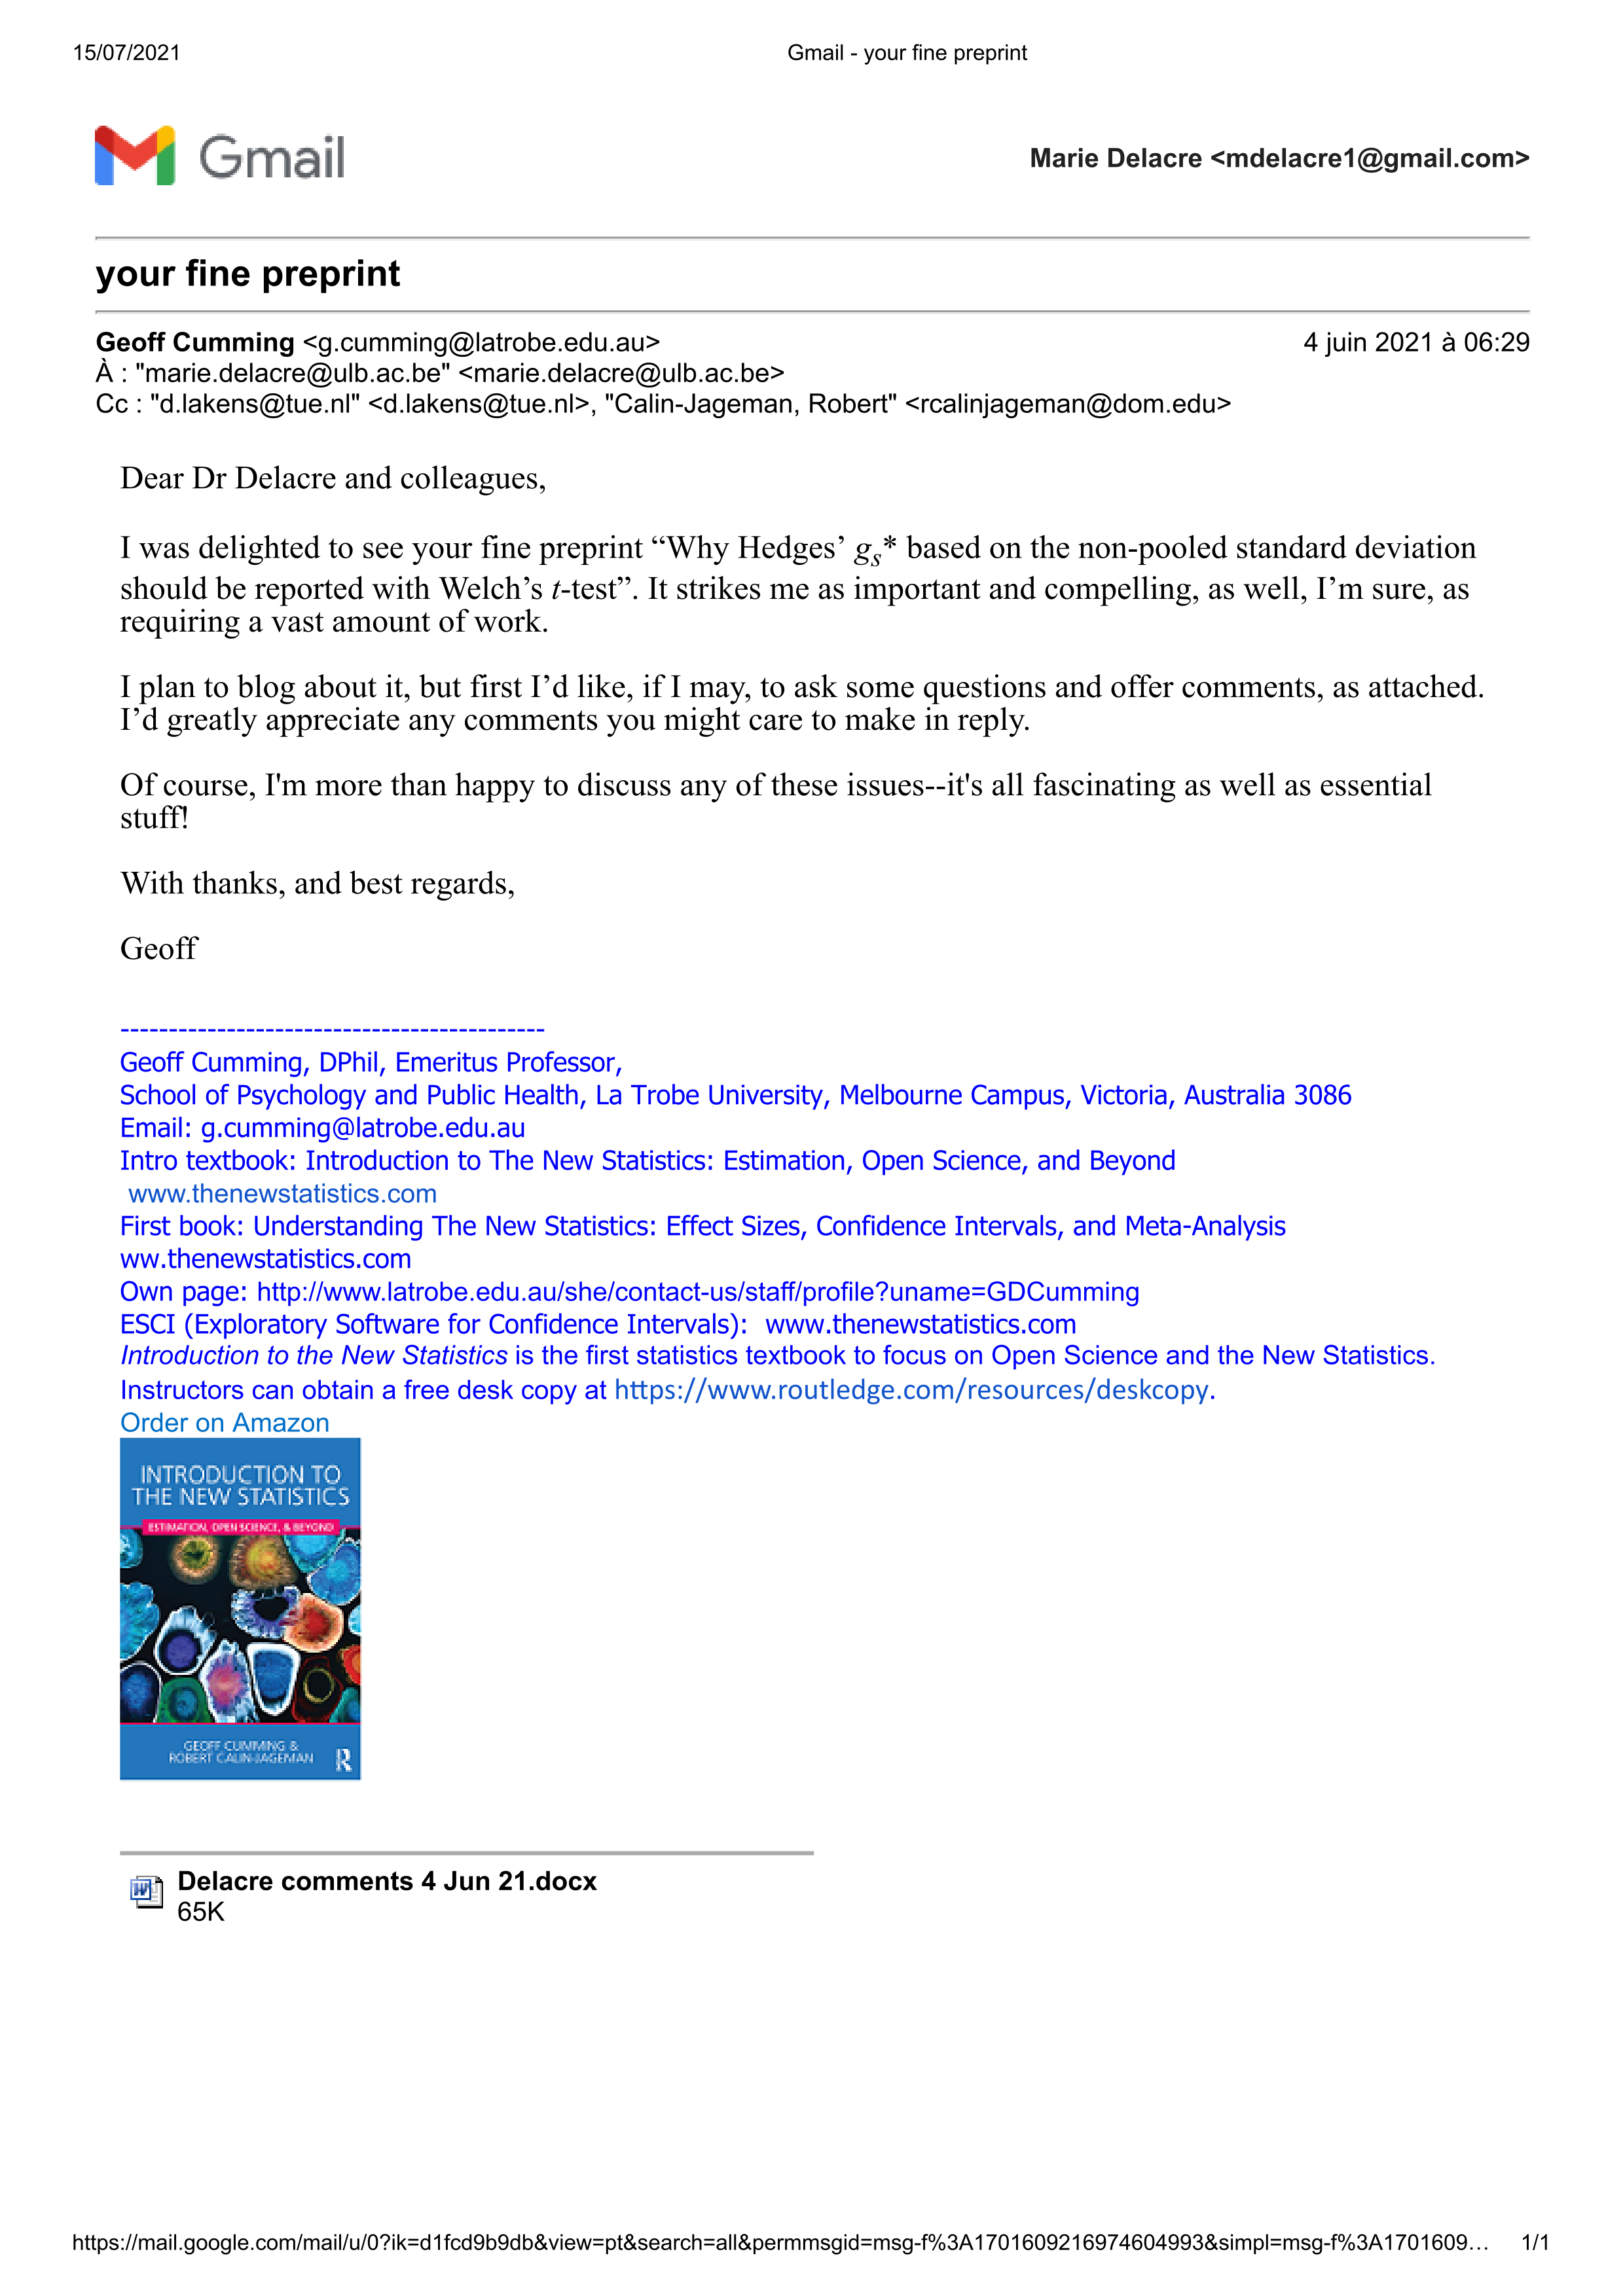
\includegraphics{C:/Users/Admin/Documents/Github projects/thesis/Chapitre 4/Echanges avec Cumming/Cummingmail1.png}
\newpage

\begin{center}\rule{0.5\linewidth}{0.5pt}\end{center}

\textbf{Why Hedges’ \(\bm{g_s^*}\) based on the non-pooled standard
deviation should be reported with Welch’s \(\bm{t}\)-test}

\underline{https://psyarxiv.com/tu6mp/}

Comments by Geoff Cumming\\
\underline{g.cumming$@$latrobe.edu.au}

4 June 2021

\textbf{Subscript \emph{s}}

I’m wondering why you use subscript \(s\) for all eight ES measures.
Yes, Cohen’s original term for the estimate was \(d_s\), but \(d\)
became the standard usage. Perhaps you use the subscript \(s\) to
indicate that the standardiser is an \(SD\) estimated from data? By
contrast \(d_\delta\), for example, would indicate that a population
value is available to use as standardiser. But in your paper there are
no such cases, so you could simplify everything by simply omitting all
those subscript \(s’\)s?

Also, that role for the subscript rules out use of it to distinguish,
for example, between \(d_p\) for pooled \(s\), and \(d_C\) for Control
group \(SD\) as standardiser. However, I know there are no
well-established conventions for such subscripts, and you need to use
‘Shieh’ as a label for those ES measures, so perhaps using name
labels (Cohen’s, etc) for all measuresâ€''as you doâ€''and dropping
all the \(s\) subscripts would be simplest.

\color{blue} I used the subscripts to indicate that the ES measure is
estimated based on a sample, but I agree that it is maybe not necessary,
so I will remove all subscripts and use labels instead.

\color{black} \textbf{Typos?}

\color{blue} Thanks for pointing all these typos out!

\color{black} p.~7, l. 139: Hedges’ \(d_s^*\) should be Cohen’s
\(d_s^*\)? \color{blue}That’s right, it should be Cohen’s \(d^*\)

\color{black} p.~8, l. 152: Use \(\sigma\) rather than
\(\sigma_{pooled}\) (twice) because here we’re assuming homogeneity of
variance, with \(\sigma = \sigma_1 = \sigma_2\) as the common population
\(SD\)? (Also Table 1, line 1 of Note.) \color{blue} \color{blue}Ok!

\color{black} p.~9, l. 3 of footnote: Not 52 but .52? (By my calcs using
\(df = 3\), \(N = 5\), and the approximate debiasing formula the value
should be .529?) \color{blue} Yes, it’s a typo, the right number is
.52 instead of 52 (see the R console below).

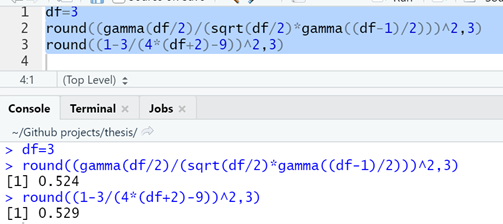
\includegraphics{C:/Users/Admin/Documents/Github projects/thesis/Chapitre 4/Echanges avec Cumming/printscreen.png}\\
\color{black} Table 3: Cohen’s \(g_s^*\) should be Hedges’
\(g_s^*\)? Also on p.~20, l. 275 (without *), and p.~30, l. 485.
\color{blue} Also true.

\color{black} \textbf{Non-normality}

It’s great that you explore non-normality, so that you are
investigating the robustness of the various ES estimators. I’d love to
see a figure showing the three example distributions you choose to
study, alongside a normal curve. Then I could have some intuitions about
how extreme they are, especially in comparison with distributions that I
might see in data I’m analysing. Thanks.

\color{blue} In the plot below, here is what the four distributions look
like when \(\mu = 0\) and \(\sigma = 1\).

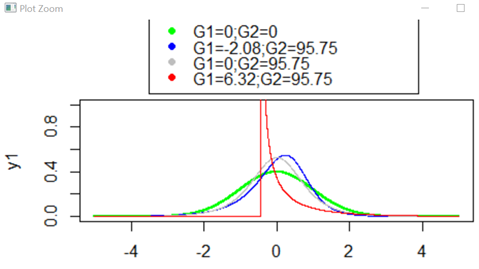
\includegraphics{C:/Users/Admin/Documents/Github projects/thesis/Chapitre 4/Echanges avec Cumming/printscreen2.png}\\
It is a nice suggestion to add a Figure in the manuscript to show the
compared distributions, I will take it into account.

Additional comment: in our simulations, we used only continuous
distributions. I think it would be interesting to test the properties of
estimators when distributions are discrete (e.g.~Likert scales) but I
have no idea how to generate such distributions in a realistic way. If
you have any suggestion, I would be more than happy to think about it
next time!

\color{brown} Yes, it would be valuable to have investigations with
discrete distributions, but I can't think of good starting points. We'd
hope for better than the normal approximation to the binomial. Maybe
start with the investigations that have been made of that, especially
with small N (Likert, as you mention).

\color{black}\textbf{Bias}

I take your point (p.~23) about the value of focusing on relative,
rather than absolute, bias (and variance) when there is a change in
measurement units. But that doesn’t happen in your investigations.

\color{blue} Well, I wrote about a “change of unit” because we use a
different standardizer for each estimator. As a consequence, each
estimator computation results in a different value in order to describe
the same amount of difference. I will clarify in the text.

\color{black} The one other reason you state for considering relative
bias is a reference, on p.~5, bottom, that Tables 1 and 2 illustrate
that “bias is directly related to the population effect size”.
That’s true for Cohen’s \(d\) in Table 1, and for \(d\) and \(d^*\)
in the top two rows of Table 2. (I’m omitting Shieh from my
commentsâ€''see below for reasons.) The debiasing that gives Hedges’
\(g\), etc, is proportional, and results in zero bias for any population
effect size. I think, therefore, that neither of the reasons you mention
for using relative bias applies for any of the \(g\) family measures in
Figures 2-9 (omitting Shieh, as I will do unless specifically
mentioned), and so I’m wondering whether seeing means (i. e., averaged
over \(\delta\) values) of relative or absolute bias would be more
informative.

\color{blue} I agree that under the normality assumption, there is no
bias for any unbiased estimator, of course. However, when the normality
assumption is not met, biases occur. In Supplemental Material 1, we
mention that when samples are extracted from heavy-tailed symmetric
distributions, this bias depends on the same parameters as the bias of
biased estimators when the normality assumption is met. It’s true that
we mainly based our decision to compute the relative bias on the
comparison between Cohen’s \(d\) (Hedges’ \(g\)) and Shieh’s \(d\)
(Shieh’s \(g\)). For example, when designs are balanced and population
variances are equal across groups, the bias of Shieh’s \(g\) is always
approximately twice smaller as the bias of Hedges’ \(g\), and its
variance is always approximately four times smaller as the bias of
Hedges’ \(g\). It gives the illusion that under this specific
configuration, Shieh’s \(g\) is less biased and variable as Hedges’
\(g\), but it is only due to what we called “a change of unit”.

Note: I explain below why I think it’s important to consider Shieh’s
\(d\) in our comparisons (even if I agree with the fact that
interpreting this measure is very hard).

\color{black} I guess I’d like to see the bias for each \(\delta\)
value. (On p.~24, line 2, you give a link to an illustration of raw bias
and variance, but I can’t find any tables or graphs of values at that
site.)

\color{blue} The graphs for raw estimators of goodness are available on
my Github account:\\
\underline{https://github.com/mdelacre/Effect-sizes/}.\\
You will find them in the following folder: ``Scripts outputs/Quality of
ES measures/Graphs/Unbiased estimators/Raw estimators of goodness/''.
The fact that you haven't found it probably means that I should
reorganize the folder, in order to make it clearer, to indicate more
clearly the Figures position in the folder or to add a read me file!

\color{brown} Thanks for the link for raw results.
https://github.com/mdelacre/Effect-sizes/ That's different from the link
in the preprint. \color{darkgray}{[}En effet, nous avions collé un
mauvais lien par erreur dans le preprint{]}.

\color{black} You say that the main purpose of the figures is to allow
comparisons between the different ES measures, rather than absolute
values for bias (and variance). Even so, knowing when bias is likely to
be absolutely small or large can inform judgments about the different ES
measures in various contexts. In Figures 2 and 3, we have
\(\sigma_1=\sigma_2\) and four versions of \(g\), all debiased. If I’m
following, the relative bias values pictured in the top rows of both
figures are averaged over \(\delta\) = 1, 2, 3, and 4. (I’m assuming
\(\sigma_1=\sigma_2=1\); correct?) \color{blue} Right! \color{black} For
the non-normal distributions, average relative bias in the best cases is
around 1-2\(\%\), so not bad. But up to around 5-10\(\%\) in some other
cases, a bit more concerning.

\color{blue} Absolutely right. However, as mentioned in the manuscript,
“we chose very extreme conditions, and we know that none of the
parametric measures of ES will be robust against such extreme
conditions”. It is therefore not surprising that \emph{all} estimators
are very large under some conditions. We could insist more on the fact
that the parametric estimators are robust only under moderate deviations
from the normality assumptions.

\color{black} It’s interesting to see that almost all the relative
bias values plotted in Figures 2-9 are positive, so in nearly all cases
the ES estimates are on average too high? If so, this may be worth
noting? (Apologies if I missed your comment on this.)

\color{blue} You’re perfectly right. There is a mathematical reason
for that (at least for symmetric distributions; it is explained in
Supplemental Material 1, in the “Preliminary note”; see below). We
did not include this note in the main manuscript because we were afraid
that it would be too technical for many psychologists, and we did not
want to complicate even more a paper that already contains many complex
concepts, but maybe we could mention this in a footnote if you think
it’s missing.

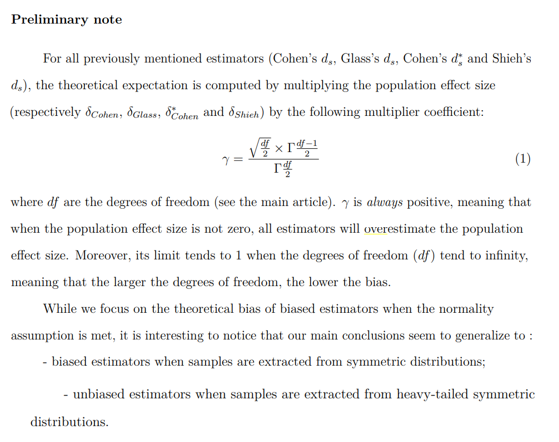
\includegraphics{C:/Users/Admin/Documents/Github projects/thesis/Chapitre 4/Echanges avec Cumming/printscreen3.png}\\
\color{black} \textbf{Variance}

For bias, the goal is zero, an unbiased estimate. For relative variance,
the smaller the better, but we don’t expect zero because we’ll
always have sampling variability in estimates of \(\delta\). I’m
finding it hard to think of a good way to get intuitions about the
empirical variances of the different ES measures, starting with the
relative values reported in Figures 2 and 3. Part of my difficulty is
that variance is a squared measure. As usual, I’d much prefer to be
able to think in terms of CIs and their lengths.

\color{blue} Thinking in terms of CIs and their lengths require to run
new simulations because we compute CIs based on the noncentral t
distribution method (the method is explained in CI.pdf, here:
https://github.com/mdelacre/Effect-sizes/tree/master/Supplemental\%20Material\%204/CI.pdf/
; the R script is available here:
https://github.com/mdelacre/Effect-sizes/blob/master/Scripts/Confidence\%20intervals/CI.R.

I have made simulations in order to compute CIs around point estimators
for all scenarios where \(\mu_1-\mu_2 = 0\) and \(\mu_1-\mu_2 = 1\).

Note that analyses on CIs would probably be very redundant with that of
the variance. I agree that the length of CIs is probably more intuitive,
but at the same time, everybody knows that the variance is a measure of
dispersion, and the greater the variance, the greater the dispersion. We
mention that our main goal is to \emph{compare} the relative bias and
variance of different estimators, and variance allows this comparison.

\color{black} The variance formulas in Tables 1 and 2 show that the
variance of \(d\) and \(g\), and the top two ES measures in Table 2, do
indeed depend on \(\delta\). To try to get a feel for the extent of this
dependence I made a quick spreadsheet of the variance formula for
Cohen’s \(d\), using the approximate formula in the second line of
Table 1. The figure below shows the percentage of variance in \(d\) that
is given by the second, \(\delta\)-dependent, term in the formula for
variance. I assumed two equal sized groups. The figure suggests that for
\(\delta<1\) only a very small \(\%\) of the variance is dependent on
\(\delta\), and for \(\delta=1\) (around 10\(\%\)) and greater, the
\(\%\) increases rapidly with \(\delta\)â€''not surprisingly, given the
\(\delta^2\) term in the formula. The \(\%\) hardly changes with sample
size, for two samples each of at least 20, as you use.

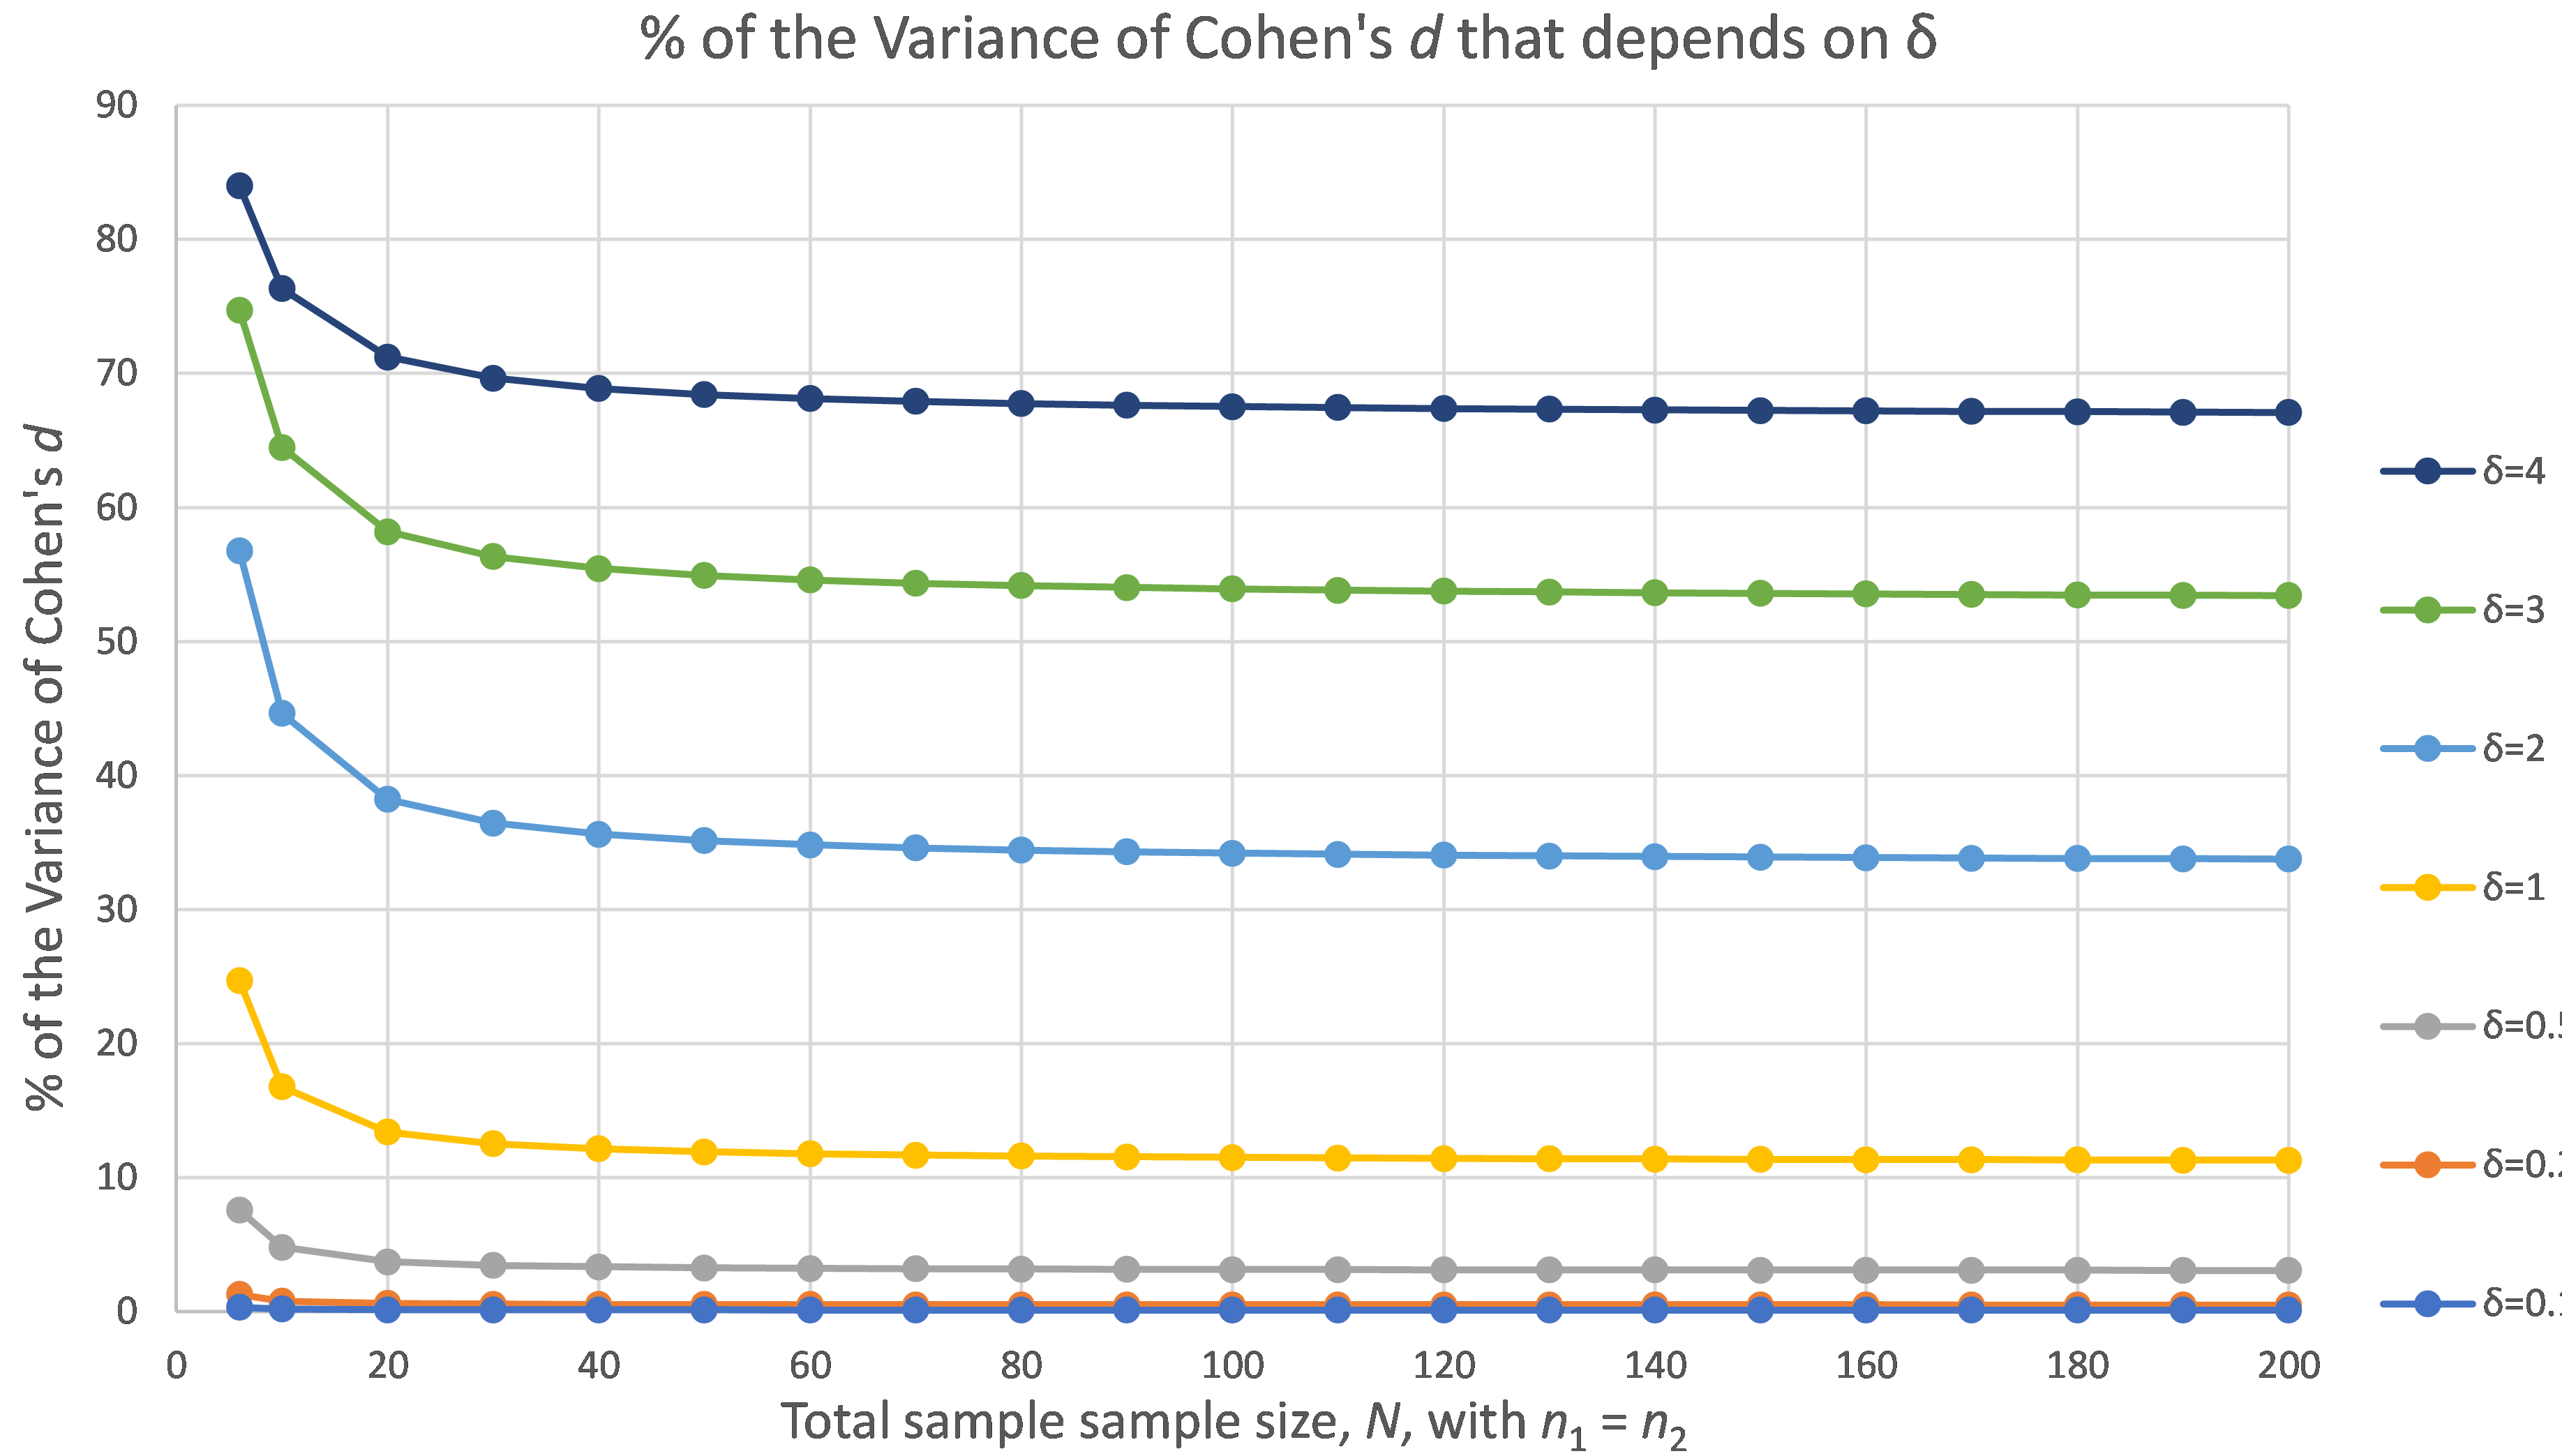
\includegraphics{C:/Users/Admin/Documents/Github projects/thesis/Chapitre 4/Echanges avec Cumming/printscreen4.png}\\
For \(\delta\) values of 1, 2, 3, and 4 (as are averaged in Figures 2,
3), the \(\%\)ages are, in round numbers, about 11, 34, 54, and 67,
respectively. I expect the \(\%\)ages for the other ES measures would
not be vastly different. Therefore the relative variance values shown in
the lower row in Figures 2 and 3 are averages over cases in which
dramatically different proportions of the variance are dependent on
\(\delta\). I think this makes it harder to get good intuitions. Values
of the variance of the estimates, rather than relative values, may be
more understandable?

\color{blue} This is a very interesting analysis. I was quite confused
about this question, and I’ve been wondering for a long time what the
best solution would be. We had many long discussions in order to decide
whether we should compute the variance or the relative variance. The
issue was indeed the fact that the variance only partly depends on
delta. Finally, we decided to compute the relative variance because we
had in mind that when \(n_1=n_2\) and \(\sigma_1=\sigma_2\), the bias
(variance) of Shieh’s \(d\) is twice smaller (four times smaller) as
the bias for Cohen’s \(d\), only because Shieh’s \(d\) is twice
smaller as Cohen’s \(d\) (see Appendix 1 in our paper). However, I
keep in mind that you argue in favor of removing Shieh's \(d\) from our
analyses.

\color{black} Taking a different approach, and considering the relative
variance values plotted in Figures 2 and 3, would it be reasonable to
say that relative \(SD\), the square root of relative variance, is the
\(SE\) used to calculate the CI on that ES estimate, expressed as a
fraction of \(\delta\), the population ES? If so, such a 95\(\%\) CI
would be about \(\pm 2 \times SE \; value \times \delta\). (Given that
the smallest total \(N\) being considered is 40, that approximation
should be reasonable? Perhaps less so for much smaller group sizes. The
asymmetry of CIs on \(d\) is actually very small unless \(N\) is very
small and \(\delta\) is large.) If that’s at least roughly correct,
then your reported values of average efficiency become indicators of the
precision of the different ES estimates. An efficiency estimate (lower
row in the figures) of, say, 0.04 (a typical low value) would correspond
approximately to \(SE=0.2\delta\) and a 95\(\%\) CI of about
\(\pm 0.4 \delta\). However, that’s very rough because the efficiency
values plotted are means of four possibly quite different values. (The
dependence of relative varianceâ€''and thus CI lengthâ€''on \(N\) is
clear in Figure 2, and can also be seen in Figure 3.)

\color{blue} This is not very clear to me. If you think this is a key
point, perhaps we could discuss it together when I will revise the
article?\\
\color{brown} It looks complicated here but, I think, mainly because
I’m trying to get approx CI info from averaged relative variance
values. It’s probably not worth considering this further, given that
somewhere in future plans may be analyses that tell us directly about CI
lengths and coverage \%ages, and likely errors (biases) in these. I’m
more than happy to discuss at revision time.

\color{black} \textbf{Shieh’s \emph{d} and \emph{g}}

I can see that including these does give a comprehensive exploration of
ES possibilities. Seeing them here led me to go back to Shieh’s
original article and my comment. You cite that comment (thank you) as
reason to doubt the value of the Shieh approach. You also point out
(p.~15, bottom) that in the base case the Shieh value is half \(d\).
This seems to me so crazy that it alone may provide sufficient reason to
dump the Shieh approach. For example, a difference of 7.5 between two IQ
means is \(d\) = 0.5, half an \(SD\). That makes sense. But Shieh would
calculate 0.25! Units of double the SD! How could we make sense of that?
How could I even attempt to justify that to students as a meaningful
standardised ES measure?

But as you say there’s more. Calculating a pooled \(SD\) weights by
sample size, for good reasons. The Shieh calculation, however
counter-weights, so the \(SD\) of the \(smaller\) group is weighted more
heavily. That’s what we need to calculate the variance, but, surely,
not a value that could justifiably be used as standardiserâ€''the units
in which to express our standardised ES.

Even more, again as you say: Simply change the \(n\)-ratio and the
\(SD\) estimate changes, so we can’t see the ES value we get as an
estimate of any readily understood population quantity.

All that seems to me more than enough reason simply to dump the Shieh
approach. Imho, it’s worth no more than a para or two to explain why
it’s not worth pursuing.

\color{blue} I get your point and I agree with all what you say. At the
same time, Shieh’s \(d\) is based on the same statistical quantity as
Welch’s \(t\)-test. By ``same quantity'', I mean that the percentage
of \(p\)-values associated with Welch's \(t\)-test below the alpha risk
exactly equals the proportion of confidence intervals around Shieh's
\(d\) that does not include 0. Our first motivation to write this paper
was to advice researchers with a measure they could use when performing
Welch’s \(t\)-test, in the continuity of our previously written
articles on the subject (“Why Psychologists Should by Default Use
Welch's \(t\)-test Instead of Student's \(t\)-test” and “Taking
Parametric Assumptions Seriously: Arguments for the Use of Welch's
\(F\)-test instead of the Classical \(F\)-test in One-Way ANOVA”). In
that context, I think it’s a bit weird to not include this effect size
estimator in our comparisons. Moreover, before running all my
simulations, I thought that this test was the best from an inferential
point of view (again, due to this mathematical relation). The study of
bias and variance reveals that even for inference, it has big flaws. For
that alone, I find it interesting to include it in the comparisons. At
the same time, we can (and we will) insist a little more on the fact
that the mathematical relation between Welch’s t-test and Shieh’s d
explains why we took this ES estimator into account, and specify at the
outset that the simulations will reveal that this measure is not very
defensible, even purely statistically speaking.

\color{black} \textbf{Results section} p.~24, ll. 356-8: moving left to
right, columns 2-4: in both figures the bias increases slightly then
decreases considerablyâ€''not “moving left to right… the larger the
bias”

\color{blue} Have you noticed that in column 4, we don’t use the same
scale as in column 2 and 3 (this is true for both Figures 2 and 3)? So
indeed the bias is larger in column 3 than in column 2, and larger in
column 4 than in column 3.

\color{brown} In some places I did note the differing vertical scales in
your figures, esp.~Column 4. But I slipped up in my comments on
interpretation of those figures. Sorry.

\color{black} p.~27, l. 403: Unequal variances. In Figure 4, what are
the variances? A single pair of values in all cases, or are the pictured
values averaged over a range of variance pairs?

\color{blue} Scenarios in Figure 4 are those where \(\sigma_1\) always
equals 1, and \(\sigma_2\) = .1, .25, .5, 2, 4 or 10, so pictured values
are averaged over a range of variance pairs. I'll mention it explicitly
in the next version to avoid confusion.

\color{black} p.~27, ll. 407-8: “when moving from left to right… the
larger the bias”. But for all Figures 4-9, except 7, bias increases
slightly (or hardly) from column 2 to 3, then drops to be smallest in
column 4.

\color{blue} Again, we don’t use the same scale in column 4
vs.~columns 2 and 3. It was mentioned p.24, l. 339.

\color{black} p.~27, ll. 408-9: “the bias of Hedges’ \(g_s\) remains
very small…” But it is often large, and in every case no smaller
than that of Hedges’ \(g_s^*\).

\color{blue} I meant that the bias of Hedges’ g remains very small
when the normality assumption is met (but this needs to be clarified
better in the sentence!).

\color{black} I’m wondering what value you use for \(\delta\) when
assessing relative bias and variance for Hedges’ \(g\). Perhaps what
you define for \(\delta_{Cohen}\) back on p.~8, l. 152? If so, that
value depends not only on the two variances, but on the two sample
sizes. So we’re estimating a population ES that doesn’t reflect any
relevant population in the world and, moreover, assuming a population ES
that changes merely because we happen to use different sample sizes.

\color{blue} What would you recommend to use? Indeed I’m using
\(\delta_{Cohen}\). Mathematically speaking, the expectation of
Hedges’ \(g\) always equals \(\delta_{Cohen}\) when both assumptions
of normality and equal population variances are met, so we compare
mean(Hedges’ g) with \(\delta_{Cohen}\) in order to compute the raw
bias. This explains why I also used \(\delta_{Cohen}\) in the
denominator when I computed the relative bias.

\color{brown} I had in mind the introduction of Cohen’s d on pp.~7-8.
We are assuming homogeneity of variance. I made a comment:\\
p.~8, l. 152: “Use \(\sigma\) rather than \(\sigma_{pooled}\) (twice)
because here we’re assuming homogeneity of variance, with
\(\sigma = \sigma_1 =\sigma_2\) as the common population \(SD\)? (Also
Table 1, line 1 of Note.)” Ok!

\(\rightarrow\) you agreed with that. So the formula, line 152, with the
square root (I’ll call that ‘the weird formula’) reduces to
\(\sigma = \sigma\). I guess I’m assuming that Cohen’s \(d\), and
also Hedges’ \(g\), are defined assuming homogeneity of variance and
their formulas use \(s_p\), the pooled value. They both estimate
\(\delta\), defined as in your (5).

Thinking further about this, I take your point. In a simulation we know
\(\sigma_1^2\) and \(\sigma_2^2\), as well as the two sample sizes, but
we know of no ‘true’ single \(\sigma\) to use in defining the
\(\delta\) we would like to use as the benchmark to assess the estimates
calculated in the simulation. Perhaps using the weird formula is the
best we can do; if anything using this means we’re bending over
backwards to minimise likely estimation error.

Perhaps you could consider shifting the weird formula from the basic
intro to Cohen’s \(d\) on pp.~7-8, where to me it doesn’t seem to
fit, and introducing it, as a sort of necessary evil, when explaining
the simulation evaluation of \(d\) and \(g\)?

\color{black} However, on p.~27, from l. 411, you say that pooling
variance estimates in this situation results in an {[}effect size{]}
estimator that “will be smaller… or larger… than it should be.”
What should it be? Doesn’t such an estimator match the definition of
\(\delta\) I refer to above? Then you make the same statement about
population values, although that would not be true if you are using the
definition of \(\delta\) I refer to aboveâ€''which is based on just such
a pooled (and weighted by sample size) population \(SD\)? Even so, your
conclusion at the top of p.~28, dismissing Hedges’ \(g\), may be
justifiedâ€''when variances differ.

\color{blue} I’m not sure that I understand your comment. Could you
please clarify? P.27, we meant that when variances are unequal across
populations, the pooled error term is not valid (because it assumes
equal population variances). When we compute the bias of Cohen’s \(d\)
in scenarios with unequal population variances, we compare an invalid
estimate with an invalid population measure of effect size. Because both
estimate and population value are invalid, the problem of Cohen's \(d\)
in case of heteroscedasticity is not revealed by the calculation of the
bias. This is actually the same explanation as p.10:

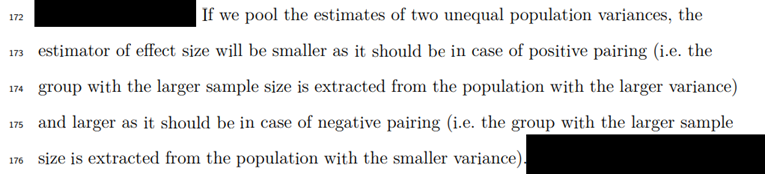
\includegraphics{C:/Users/Admin/Documents/Github projects/thesis/Chapitre 4/Echanges avec Cumming/printscreen5.png}\\
\color{brown} Given your explanation about using the weird formula, I
think I now understand what you were getting at. Your statement that the
estimate and the population measure (calculated using the weird formula)
are both invalid expresses the problem that there’s probably no good
way to calculate the population measure when variances are unequal. No
sensible way to specify what the estimate should be estimating. Indeed!

Of course, if we try to avoid the double invalidity you point to by
simply averaging the two different \(\sigma\) values, we get the \(d^*\)
and \(g^*\) estimators. These may solve the unequal \(n\) problem of the
weird formula, but still have problems (in my view, severe problems) in
terms of interpretability.

\color{black} p.~28, l. 422: “parameters that we cannot control…”.
You include the \(n\)-ratio, which is true if, for example, we are
meta-analysing past research. But in many cases a researcher chooses
sample sizes, and your investigations are likely to lead to useful
advice about choice of sample sizes.

\color{blue} I think it’s partly true. About the bias, the larger the
control group size, the lower the bias. About the variance, it’s a bit
more complex: in Supplemental Material 1 we write that when the
normality assumption is met “The variance always decreases when the
control and/or the experimental group increases. The benefit of adding
subjects in the control, in the experimental, or in both groups, in
order to reduce the variance, varies as a function of the \(SD\)-ratio
and the population effect size. The only situation where it is optimal
to maximize the experimental group is when \(\sigma_e>\sigma_c\) and
\(\delta_{Glass}\approx 0\). Most of the time, it is more efficient to
maximize the control groups (e.g.~anytime \(\sigma_e<\sigma_c\), and
when \(\delta_{Glass}\) is very large) or to uniformly add subjects in
both groups (e.g.~when \(\sigma_e>\sigma_c\) and \(\delta_{Glass}\) is
neither null nor huge)” (This is a summary but you can see more
details and figures here:
https://github.com/mdelacre/Effect-sizes/blob/master/Supplemental\$\%\(20Material\)\%\(201/Theoretical\)\%\(20Variance\)\%\(20of\)\%\(20all\)\%\(20estimators\)\%\(20as\)\%\(20a\)\%\(20function\)\%\(20of\)\%\(20population\)\%\$20parameters.pdf
).

As we can see in this summary, recommendations about sample sizes would
be different as a function of \(SD\)-ratio and most of the time, we
don’t know the \(SD\)-ratio in advance. But thanks for pointing this
out, it probably deserves at least a footnote!

\color{black} \textbf{Discussion}\\
I think your three purposes of ES estimators (pp.~3-4) are spot on. Your
three desirable properties are indeed the desirable statistical
properties, but I’d list interpretability in the research context as
the first essential property. If we don’t have interpretability for a
particular standardised ES estimator then we shouldn’t be using it.

\color{blue} Theoretically speaking, I agree with you. But practically,
as I've mentioned before, I'm not sure if it's a good idea to rule out
an estimator that has such a direct connection to Welch's \(t\)-test. It
is probably possible to introduce things differently, to explain in
advance that the Shieh’s \(d\) is not desirable (and to add that even
from an inferential point of view, it has big flaws).

Apart for that, you’re right, interpretability should be our first
priority. For example, if we don’t have an interpretable measure, we
cannot use it in order to make informative null hypothesis (e.g.~when
performing equivalence test). However, I’m a bit concerned with the
fact that interpretability and good inferential properties seem so
difficult to reconcile. How could we interpret an estimator correctly if
it is very biased? This makes me very reserved about Glass's \(d\).

\color{black} I note these recommendations:

\begin{enumerate}
\def\labelenumi{\arabic{enumi}.}
\tightlist
\item
  p.~10: “Because the assumption of equal variances… is rarely
  realistic… both Cohen’s \(d\) and Hedges’ \(g\) should be
  abandoned…”. I think that’s arguable. I’m not convinced that
  assumption is rarely realistic. The assumption is very often made, for
  example, I think, in medicine when calculating SMD. I suspect a large
  proportion of Cochrane systematic reviews include meta-analyses that
  make this assumption. Of course that doesn’t make it justified in
  every situation, but I suggest the emphasis should be on informed
  judgment in context rather than simply abandoning these ES estimates.
\end{enumerate}

\color{blue} Perhaps do we need to be more nuanced in asserting this.
However, there are many authors who believe that the assumption of
homogeneity of variances often does not hold (see for example Erceg-Hurn
\& Mirosevich, 2008; Zumbo \& Coulombe, 1997). In a previous paper
(Delacre et al.~2017) we develop many reasons why we think equal
population variances are very rare in practice.

Moreover, it’s very hard to check for the homogeneity of variances
assumption, because:\\
* the assumption is about population parameters that we don’t know
(\(\sigma_1\) and \(\sigma_2\));\\
* inferential statements about the homogeneity of variances assumptions
based on assumptions tests often lack power to detect assumption
violations.

Finally, when we look at figures, we notice that when variances are
equal across groups, Cohen’s \(g\) and Cohen’s \(g^*\) are either
identical (Figure 2) or very close (Figure 3). The only exception is
when both skewness and kurtosis are very large (as reminder, we used
different scale in the fourth column in comparison with all other
columns). Most of the time, there is therefore little cost in choosing
Cohen’s \(d^*\) by default. On the contrary, Cohen's \(d\) cannot be
used in case of heterogeneity of variances. -- Delacre, M., Lakens, D.,
\& Leys, C. (2017). Why psychologists should by default use 521
Welch’s t-test instead of Student’s t-test. International Review of
Social Psychology, 522 30 (1), 92â€``101.
https://doi.org/10.5334/irsp.82

-- Erceg-Hurn, D. M. \& Mirosevich, V. M. (2008). Modern robust
statistical methods: An easy way to maximize the accuracy and power of
your research. American Psychologist, 63(7), 591. DOI: https://doi.
org/10.1037/0003-066X.63.7.591

-- Zumbo, B. D. \& Coulombe, D. (1997). Investigation of the robust
rank-order test for non-normal populations with unequal variances: The
case of reaction time. Canadian Journal of Experimental Psychology/Revue
Canadienne de Psychologie Expérimentale, 51(2), 139. DOI: https://doi.
org/10.1037/1196-1961.51.2.139

\color{black}

\begin{enumerate}
\def\labelenumi{\arabic{enumi}.}
\setcounter{enumi}{1}
\tightlist
\item
  pp.~17-18: You note the wide criticism of Cohen’s \(d^*\) (and by
  implication Hedges’ \(g^*\)) because the standardiser is not the
  \(SD\) of an existing relevant population. You state that, even so,
  these estimators have very good inferential properties. Grissom and
  Kim (2012), referring to this averaging of variances, state that we
  “are estimating the \(\sigma\) of a hypothetical population… which
  is a concern for some … but not others” (p.~72). I tend towards
  the concerned end of that range, but I know there are arguments in
  favour of using the square root of the average of two different
  variances as standardiser. Maybe it can sometimes be possible to give
  a reasonable interpretation using such a strange standardiser. Think
  of two overlapping normal curves with different \(SD\)s: What \(SD\)
  unit is best for expressing the difference between the two means? Does
  it make sense to use a compromise between those two \(SD\) values?
  Again, this should be recognised as a judgment call, and lack of
  interpretability in context should never be over-ruled by good
  statistical properties.
\end{enumerate}

\color{blue} I find this convincing (especially the fact that
interpretability should never be over-ruled by good statistical
properties) and will have to think about a better way to introduce this
estimator.

\color{black}

\begin{enumerate}
\def\labelenumi{\arabic{enumi}.}
\tightlist
\item
  p.~28, l. 424: “We do not recommend using {[}Glass’s \(g\){]}.”
  I suggest that Glass vs something else is the choice that most clearly
  should be based on the context. Does it make sense to use the \(SD\)
  of one group as the standardiser? If so, we should do so, unless there
  are very strong reasons against. We should use choice of sample sizes
  and perhaps other strategies to minimise any disadvantage of the Glass
  ES estimate. You make several observations that can help, mainly that
  increasing the control group sample size is desirable.
\end{enumerate}

\color{blue} As previously mentioned, we need to increase the control
group in order to reduce the bias, but sometimes, we need to increase
the experimental group in order to reduce the variance. This makes
recommendations about sample sizes very complicated.

\color{black}

\begin{enumerate}
\def\labelenumi{\arabic{enumi}.}
\setcounter{enumi}{1}
\tightlist
\item
  p.~30, l. 473: “We recommend using Hedges’ \(g^*\)… ” You
  state some strong advantages of this ES estimator, but I remain
  hesitant because of the possible interpretive difficulty, given its
  standardiser.
\end{enumerate}

Overall, you provide a wonderful range of detailed findings. I’d love
to see you develop the discussion, drawing further on those findings, in
a way that guides a researcher’s likely full decision sequence. For
example, first, do we have some relevant population \(SD\) value? If so,
use this as standardiser. If not, Glass or something else, considering
the context? If not Glass, homogeneity of variance or not? Then, can we
improve the precision of estimation of our chosen standardiser by, for
example, pooling over studies, or meta-analysing our data with past
research? Meaningfulness and interpretability in the context should
always be the primary consideration.

The great value of your findings is then to help us be specific about
the trade-offs. If I choose Glass, how large is the likely bias? If only
a few \(\%\) I might be prepared to tolerate that, or I might consider a
data transformation to reduce the departure from normality. (Perhaps a
log transform of RT data?) Of course, all such choices should where
possible be made in advance of seeing the data, when formulating the
data analysis plan to be preregistered.

\color{blue} This is a set of considerations that I will have to take
into account when I rework my article in September. If you're ok with
that, I'd love to show you our next draft before submitting it.

\color{brown} I'd be more than happy to comment on future drafts, in due
course. Or to discuss any of these fascinating issues!

\color{black} Earlier I made a very sketchy attempt to estimate roughly
what CI length might be, given your relative variance results. You refer
(e.g., p.~17, l. 253) to “very good inferential properties”.
That’s highly relevant, but I suggest CI length and coverage should be
central issues in assessing the inferential effectiveness of any
estimator. Then, when considering some judgment call, I could weigh up
any price there might be to pay in terms of a longer CI for one of the
options under consideration, or a slight departure from 95\(\%\)
coverage. No doubt investigation of CI length and coverage would be a
further project, although perhaps you could derive from your variance
results some relevant guidance based on CIs?

Ideally, we’d like to see the performance of CIs based on non-central
\(t\) distributions, and also bootstrapped CIs, for the various
estimators and conditions you investigate. Ideally, again, we could then
weigh up the various choices, with some idea as to the cost in terms of
bias or CI length or coverage error of a choice that offers superior
interpretabilityâ€''which should always be paramount.

\color{blue} As mentioned above, I already computed CIs for all the
conditions, based on non-central \(t\) distributions. However, I haven't
analyzed them yet but I could use them in order to compute the coverage
probability and CI length. Therefore these comments could be part of the
“further studies” section, and be the subject of a second paper.

\color{black} Overall, your investigations give us highly valuable
findings to guide such discussions.

\textbf{Title}

Current title: “Why Hedges’ \(g_s^*\) based on the non-pooled
standard deviation should be reported with Welch’s \(t\)-test”.

Why mention that \(t\)-test? Yes, it fits with your message that the
assumption of homogeneity of variance should be avoided, but it’s
hardly mentioned in the paper, and if an ES estimate and CI are reported
there’s no need to report or even mention any \(t\)-test. I would
argue that it’s much better to avoid doing so.

More positively, your investigations warrant broader recognition and
description. Perhaps something like: “\(d\)-family standardised effect
size estimators: Interpretability, bias, efficiency, and robustness”
“\(d\)-family standardised effect sizes: Bias, efficiency, and
robustness” “Cohen’s \(d\) and related effect size estimators:
Interpretability, bias, precision, and robustness” {[}my current
favourite; assumes some discussion of CIs{]} “Cohen’s \(d\),
Hedges’ \(g^*\), and related effect size estimators: Interpretability,
bias, precision, and robustness” {[}includes the largest set of terms
likely to be used in an online search{]}

\color{blue} We wanted to mention \(t\)-test because this answering the
question many people asked us: Which effect size should I report for
Welch’s \(t\)-test. Yes, the paper discusses more, adding
Interpretability, bias, precision, and robustness is a good addition.
What do you think about: “Arguments to use the Hedges’\(g_s^*\) with
the Welch’s \(t\)-test: an investigation of interpretability, bias,
precision, and robustness of d-family effect sizes”?

\color{brown} As I said in the blog post, \color{darkgray} {[}Voir lien
vers le blog post{]} \color{brown} I’m not convinced that Welch’s
\(t\)-test deserves mention, even though you have made a strong case for
using that form of the \(t\)-test in your earlier paper. If people ask
‘which \(ES\)?’ I’d answer that they need to make a judgment in
context, partly guided by your robustness resultsâ€''but I’ve said all
that in the post.

I know that you make a general recommendation that, when variances are
or may be unequal, we should use Hedges’ \(g^*\), and, separately,
Welch’s \(t\)-test, but I don’t see any other link between the two.

Your Equation (10), p.~15, expresses the very strong link between
Welch’s \(t\) and Shieh’s \(d\). Somewhere I’ve read a statement
that the CI on Shieh’s \(d\) corresponds with Welch’s \(t\) test in
the sense that the two give the same \(p\) values, tho’ I can’t find
that statement in Shieh (2013) or in your preprint or supp
materialâ€''sorry if I’ve missed it. However, I’d expect that the CI
on your recommended Hedges’ \(g^*\) and Welch’s \(t\) would not give
the same \(p\) values. If that’s correct, we have one more reason not
to link the two together, for example in the title.

\color{black} Grissom, R. J., \& Kim, J. J. (2012). \emph{Effect sizes
for research}, \(2{nd}\) ed.~New York: Routledge.

\color{brown} It's nice to see a bunch of likes and retweets to the
tweet about the blog post. \color{darkgray} {[}See
\underline{https://twitter.com/TheNewStats/status/1405386935074496512}{]}

\color{brown} There's a useful comment (link below) from Brenton Wiernik
about relevant work by Doug Bonnett. Very likely you know this, tho'
it's new to me. I'd better have a squiz.

Cheers, Geoff\\
\color{black}
------------------------------------------------------------

\newpage

\hypertarget{annexe-d-a-voir-si-erratum-du-chp-5}{%
\subsection{Annexe D: A VOIR SI ERRATUM DU CHP
5?}\label{annexe-d-a-voir-si-erratum-du-chp-5}}
\end{appendix}
